\section{Spineless Traversal}

Spineless Traversal is such an algorithm.
Unlike Double Dirty Bit,
  Spineless Traversal can jump directly to the next dirty node
  without accessing any auxiliary nodes;
  as a result, it suffers dramatically fewer cache misses
  than Double Dirty Bit.
Achieving this requires a more computationally-heavy approach,
  storing all dirty nodes in a priority queue
  and maintaining the correct traversal order
  using an order maintenance data structure.
Spineless Traversal's savings in cache misses
  outweigh the greater computational requirements
  of these data structures.

\subsection{The Priority Queue}

Spineless traversal is conceptually simple.
Each node field in the layout tree is assigned a label,
  indicating its position in a layout trace\ref{par:trace}.
Node fields are placed in a priority queue when dirtied,
  with the label used as their priority.
To perform an incremental layout,
  node fields are popped from the priority queue and recomputed,
  with dependent fields
  added back to the priority queue as they get dirtied,
  until the priority queue is empty.
Because the priority queue pops node fields with smaller labels first,
  Spineless Traversal respects the dependency order of layout.
Since only dirty nodes are ever pushed or popped from the priority queue,
  no auxiliary nodes are accessed.

We use a min-heap for our priority queue,
  which is cache-friendly and requires relatively few operations
  for each push and pop.
Moreover, the queue is typically small:
  while there are typically thousands of nodes,
  with each node having approximately 50 fields,
  the priority queue typically contains less than 1000 fields,
  and for the most latency-critical interactions,
  like hovers or drags, it can contain 100 or fewer.
With such a small size, a priority queue push/pop requires
  5--10 label comparisons,
  which can be performed in roughly the time
  for one or two L2 cache misses
  in our optimized implementation.
Since there are typically \emph{far} more auxiliary than dirty nodes,
  this means Spineless Traversal performs much faster
  than Double Dirty Bit.

\subsection{Order Maintenance}

The key to Spineless Traversal is maintaining the labels.
The issue is that layout nodes are added and removed over time;
  labels need to be comparable,
  but it also needs to be possible
  to add new labels between existing ones,
  arbitrarily.
Following SAC~\cite{SAC},
  spineless traversal achieves this using
  an \emph{order maintenance} data structure.
First introduced by \citet{OM},
  order maintenance is a data structure
  that maintains a totally ordered set of objects
  while allowing objects
  to be added and removed from the order arbitrarily.
Crucially, both adding/removing and comparing nodes
  takes $O(1)$ time.
Abstractly, order maintenance provides the following API:

\begin{enumerate}
\setlength{\itemindent}{8em}
  
\item[$\mathsf{Compare}(p, q)$] Decides whether $p$ or $q$ comes first in the order (or are equal).
\item[$\mathsf{Head}()$] Returns the first object of the order.
\item[$\mathsf{Create}(p)$] Creates and returns a new object right after $p$.
\end{enumerate}

\noindent
Deleting OM objects is also possible; however,
  our implementation does not.

Our implementation is based on that by \citet{SOM},
  which uses a two-level structure with
  a double-linked list of double-linked lists.
Objects are represented by nodes in the lower-level lists.
Both levels are ordered;
  the total order traverses lower-level lists in order,
  in the order dictated by the higher-level list.
Each object (node in the lower-level list)
  maintains a pointer to its higher-level list cell;
  two objects are in the same low-level list
  if they have the same higher-level pointer.
To allow fast comparisons between nodes,
  both low-level and high-level list cells store
  an unsigned integer of fixed size
  (in our implementation, 32~bits)
  called labels.
Within both lists, node labels are strictly increasing;
  this makes comparisons fast.
Specifically, comparison has two cases:
  the two objects can be in the same low-level list,
  in which case their labels can be compared,
  or in different ones, in which case
  their parents' labels can be compared.
This comparison operation is
  the bulk of the Spineless Traversal time
  so its simplicity is essential;
  Section~\ref{sec:opt} discusses how we
  micro-optimize it in our implementation.

To create an object inside an order maintenance structure,
  a new lower-level list cell is created
  whose label is the average of the two neighboring labels.%
\footnote{
  When creating a node after the last node,
  the maximum representable number is used as the larger number.
}
If the two labels differ by exactly 1, however,
  this becomes impossible (a label would be repeated).
In this case, the data structure re-balances itself,
  evenly reassigning labels to existing objects.
This process might
  create a new higher-level list cell
  to split a lower-level list in two,
  ensuring a sufficiently large gap between its cells.
Rebalancing is algorithmically tricky
  but is not a significant time sink in our use case,
  so we do not detail re-balancing here;
  details can be found in \citet{SOM}.

\begin{figure}
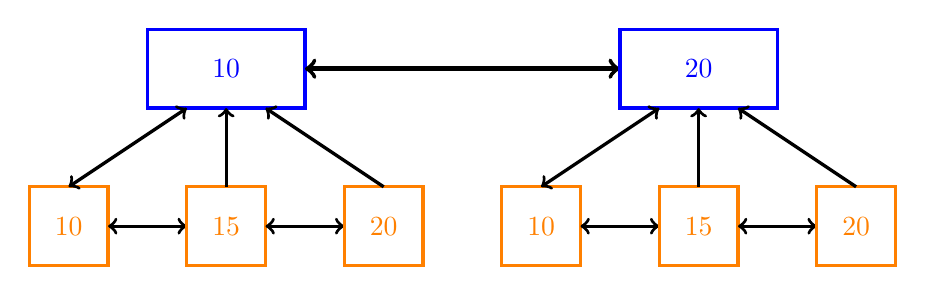
\begin{tikzpicture}
\draw[blue, very thick] (1.5,0) rectangle (3.5,1) node[pos=.5]{10};
\draw[ultra thick, <->] (3.5,0.5) -- (7.5,0.5);
\draw[blue, very thick] (7.5,0) rectangle (9.5,1) node[pos=.5]{20};

\draw[orange, very thick] (0, -2) rectangle (1,-1) node[pos=.5]{10};
\draw[very thick, <->] (0.5,-1) -- (2,0);
\draw[very thick, <->] (1,-1.5) -- (2,-1.5);
\draw[orange, very thick] (2, -2) rectangle (3,-1) node[pos=.5]{15};
\draw[very thick, ->] (2.5,-1) -- (2.5,0);
\draw[very thick, <->] (3,-1.5) -- (4,-1.5);
\draw[orange, very thick] (4, -2) rectangle (5,-1) node[pos=.5]{20};
\draw[very thick, ->] (4.5,-1) -- (3,0);

\draw[orange, very thick] (6, -2) rectangle (7,-1) node[pos=.5]{10};
\draw[very thick, <->] (6.5,-1) -- (8,0);
\draw[very thick, <->] (7,-1.5) -- (8,-1.5);
\draw[orange, very thick] (8,-2) rectangle (9,-1) node[pos=.5]{15};
\draw[very thick, ->] (8.5,-1) -- (8.5,0);
\draw[very thick, <->] (9,-1.5) -- (10,-1.5);
\draw[orange, very thick] (10, -2) rectangle (11,-1) node[pos=.5]{20};
\draw[very thick, ->] (10.5,-1) -- (9,0);

\end{tikzpicture}
\caption{An Order Maintenance data structure. The blue node represent the higher level doubly linked list, and each node store a lower level doubly linked list, denoted by the orange node. Lower level node also store a pointer to the higher level node. Each node additionally hold an unsigned integer, label, such that inside a single list the node earlier have a strictly smaller label then the node later.}
\label{fig:om}
\end{figure}

\subsection{Bulk insertion and deletion}

\label{sec:tree-insertion}
Bulk insertions into the layout tree are common,
  often due to a ``lazy loading'' pattern:
  a ``shell'' web page loads first and shows a loading indicator;
  then the ``content'' loads and is inserted into the page
  as a single large subtree.
This pattern is encouraged by frameworks like React,
  and can occur in several stages, with a ``shell''
  first inserting ``subshells'' which
  themselves load subcomponents in turn.
Efficiently inserting the large subtree
  requires special care in Spineless Traversal.

The basic issue is that all fields of all nodes in the subtree
  need to have them and their OM objects initialized,
  yet we also want subtree insertion to be fast.
Our solution adds these ``initialization passes''
  as special elements in the priority queue.%
\footnote{
  Just enqueueing all fields of all nodes in the subtree
    is not a good idea---it will create a large queue with slow queue operations.
  In our experiments, this often took the queue
    from tens to thousands of members,
    leading to a small integer slowdown.
}
In other words, the priority queue can contain
  not only $(n, v)$ pairs for a dirtied field
  but also $(r, p)$ fields pointing to the root $r$
  of an entire subtree that needs to be initialized
  for pass $p$.
When a subtree $T$ is inserted, each pass for it is enqueued;
  the Order Maintenance object for that
  is created after the OM of the last field
  initialized by $P$ in $T$'s previous sibling or parent.
In this way, we maintain the consistency of incremental layout 
  with from-scratch layout.
\footnote{
  An edge case is inserting a subtree into
    a subtree that itself has not yet been laid out.
  In this case no further actions need to be taken,
    since both subtrees will be visited together.}

When one of these $(r, p)$ elements is popped from the queue,
  the pass $p$ is performed on the whole subtree under $r$,
  creating all necessary order maintenance nodes.
Since all fields in newly-created nodes are initially dirty,
  performing this pass will not enqueue any fields
  in the priority queue,
  meaning that no priority queue operations
  need to be performed.
Likewise, since all data accesses are local,
  no existing nodes will refer to any newly-inserted node
  except the root node,
  so no nodes need to be dirtied when running $p$ on the subtree.
This means that, when initializing a subtree,
  no priority queue operations or dirty bit propagations
  need to be performed,
  which makes subtree insertion faster.
(However, order maintenance objects still need to be created,
  meaning that, despite these optimizations,
  Spineless Traversal is typically
  slower than Double Dirty Bit
  for subtree insertion.)

When deleting a subtree,
  some nodes in the subtree may
  already be in the priority queue;
  for example, this can happen if
  a subtree is inserted and then later deleted.
To avoid unnecessary recomputation,
  we add a ``deleted'' bit to each node
  and skip recomputing such node.%
\footnote{Those nodes are ref-counted and the memory will be reclaimed at the right moment.}